\documentclass[conference]{IEEEtran}
\usepackage{graphicx}
\usepackage{amsmath}
\usepackage{cite}
\usepackage{listings}
\usepackage{xcolor}

% Code style
\lstdefinestyle{mystyle}{
    backgroundcolor=\color{gray!10},   
    commentstyle=\color{green!50!black},
    keywordstyle=\color{blue},
    numberstyle=\tiny\color{gray},
    stringstyle=\color{orange},
    basicstyle=\ttfamily\footnotesize,
    breaklines=true,
    captionpos=b,
    numbers=left,
    numbersep=5pt,
    showspaces=false,
    showstringspaces=false,
    showtabs=false,
    tabsize=2
}
\lstset{style=mystyle}

\title{Genetic Algorithm Approach to the Travelling Salesperson Problem}

\author{
    \IEEEauthorblockN{Ignat Bojinov}
    \IEEEauthorblockA{StFX \\
    2025fve@stfx.ca}
}

\begin{document}
\maketitle

\section{Introduction}
\subsection{What is the problem?}
The Traveling Salesman Problem (TSP) is a classical NP-hard problem in combinatorial optimization, important in theoretical computer science and operations research. It asks a deceptively simple question: 

\emph{``Given a list of cities and the distances between each pair of cities, what is the shortest possible route that visits each city exactly once and returns to the origin city?''}

\subsection{Small review}
Over the decades, various methods have been developed for solving TSP. Exact approaches include branch-and-bound and dynamic programming, but these scale poorly. Approximation and heuristic methods such as nearest neighbor and 2-opt are widely used for smaller problems. Metaheuristics such as Genetic Algorithms (GA), Simulated Annealing, and Ant Colony Optimization have shown good performance on medium to large instances. In particular, GAs are often chosen because of their flexibility and ability to balance exploration and exploitation of the search space \cite{wikiTSP}.

\section{Problem Description}
\subsection{What is TSP?}
Formally, the TSP can be expressed as finding a Hamiltonian cycle of minimum length in a weighted complete graph where nodes represent cities and edge weights represent distances. In this assignment, distances are Euclidean, calculated from provided 2D coordinates in JSON-formatted datasets.

\section{Algorithm Description}
\subsection{How was the GA implemented?}
The GA implementation follows the standard framework but is adapted for TSP in Python.

\paragraph{Initialization}
The population is generated as random permutations of city IDs:
\begin{lstlisting}[language=Python]
def initial_population(pop_size, cities):
    city_ids = list(cities.keys())
    population = []
    for _ in range(pop_size):
        route = city_ids[:]
        random.shuffle(route)
        population.append(route)
    return population
\end{lstlisting}

\paragraph{Fitness function}
Fitness is defined as the total Euclidean distance of the route (shorter routes are better):
\begin{lstlisting}[language=Python]
def route_dist(route, cities):
    dist = 0
    for i in range(len(route)):
        city_a = cities[route[i]]
        city_b = cities[route[(i + 1) % len(route)]]
        dist += euclid_dist(city_a, city_b)
    return dist
\end{lstlisting}

\paragraph{Selection}
Tournament selection ( \texttt{sorry\_loosers}) picks the best out of a random subset:
\begin{lstlisting}[language=Python]
def sorry_loosers(population, cities, k=5):
    fight = random.sample(population, k)
    fight.sort(key=lambda route: route_dist(route, cities))
    return fight[0]
\end{lstlisting}

\paragraph{Crossover}
Order crossover preserves a slice from one parent and fills the rest from the other:
\begin{lstlisting}[language=Python]
def crossover(daddy, mommy):
    size = len(daddy)
    start, end = sorted(random.sample(range(size), 2))
    child = [None] * size
    child[start:end] = daddy[start:end]
    mommy_el = [c for c in mommy if c not in child]
    pos = 0
    for i in range(size):
        if child[i] is None:
            child[i] = mommy_el[pos]
            pos += 1
    return child
\end{lstlisting}

\paragraph{Mutation}
Swap mutation randomly exchanges two cities with probability equal to the mutation rate:
\begin{lstlisting}[language=Python]
def ninja_turtles(route, mutation_rate=0.01):
    route = route[:]
    for i in range(len(route)):
        if random.random() < mutation_rate:
            j = random.randint(0, len(route)-1)
            route[i], route[j] = route[j], route[i]
    return route
\end{lstlisting}

\paragraph{Next generation with elitism}
The best solution is preserved, and the rest are produced by selection, crossover, and mutation:
\begin{lstlisting}[language=Python]
def bright_future(population, cities, elite_size=1, mutation_rate=0.01):
    population.sort(key=lambda r: route_dist(r, cities))
    natural_selection = population[:elite_size]
    while len(natural_selection) < len(population):
        daddy = sorry_loosers(population, cities)
        mommy = sorry_loosers(population, cities)
        child = crossover(daddy, mommy)
        child = ninja_turtles(child, mutation_rate)
        natural_selection.append(child)
    return natural_selection
\end{lstlisting}

\subsection{Enhancements and modifications}
Several modifications were included in this implementation:
\begin{itemize}
    \item \textbf{Elitism:} Ensures best individuals survive to the next generation.
    \item \textbf{Tournament selection:} Stronger parent competition than random selection.
    \item \textbf{Parameter variety:} Different population sizes, mutation rates, and generations tested.
    \item \textbf{Visualization:} Added convergence plots and final-route diagrams for interpretability.
\end{itemize}

\section{Analysis Plan}
The GA was compared against:
\begin{itemize}
    \item \textbf{Baseline:} Greedy nearest neighbor heuristic.
    \item \textbf{Instances:} berlin52 (small), a280 (medium), pcb442 (large).
    \item \textbf{Configurations:} Two mutation rates (0.01, 0.05).
    \item \textbf{Statistics:} 10 runs each → mean, standard deviation, worst/best distances.
\end{itemize}

\section{Results and Discussion}
\subsection{Numerical Results}
Table~\ref{tab:results} summarizes the GA performance against nearest neighbor.

\begin{table}[h]
\centering
\caption{Comparison of GA vs. Nearest Neighbor}
\label{tab:results}
\begin{tabular}{|l|l|r|r|r|}
\hline
Instance & Method & Best Dist & Mean Dist & Std Dev \\
\hline
berlin52 & NN  & 8980.9  & -      & - \\
berlin52 & GA (0.01) & \textbf{8648.0} & 9382.7 & 457.7 \\
berlin52 & GA (0.05) & 12815.0 & 13596.5 & 643.3 \\
\hline
a280     & NN  & 3148.1  & -      & - \\
a280     & GA (0.01) & \textbf{19476.3} & 20100.6 & 411.4 \\
a280     & GA (0.05) & 25671.3 & 26283.8 & 364.2 \\
\hline
pcb442   & NN  & 61984.0 & -      & - \\
pcb442   & GA (0.01) & \textbf{517358.0} & 529792.4 & 7857.7 \\
pcb442   & GA (0.05) & 629252.3 & 642718.7 & 7137.2 \\
\hline
\end{tabular}
\end{table}

\subsection{Interpretation}
Several trends emerged:
\begin{itemize}
    \item For \textbf{berlin52}, the GA with low mutation rate outperformed nearest neighbor, achieving shorter routes (8648 vs. 8981). However, higher mutation degraded results.
    \item For \textbf{a280}, GA produced routes much longer than nearest neighbor (19k–26k vs. 3.1k). This indicates the GA struggled to scale.
    \item For \textbf{pcb442}, the GA completely failed to compete (517k–629k vs. 62k). The algorithm likely got trapped in poor local minima and could not exploit the search space effectively.
    \item Runtime scaled significantly: $\sim$24s for berlin52, $\sim$187s for a280, and $\sim$376s for pcb442.
\end{itemize}

\subsection{Statistical Observations}
The GA displayed moderate variability (std. dev. 364–7857), meaning results are not deterministic but consistent within ranges. Mutation rate 0.01 consistently outperformed 0.05, highlighting the risk of excessive exploration.

\subsection{Visual Results}
\begin{figure}[h]
    \centering
    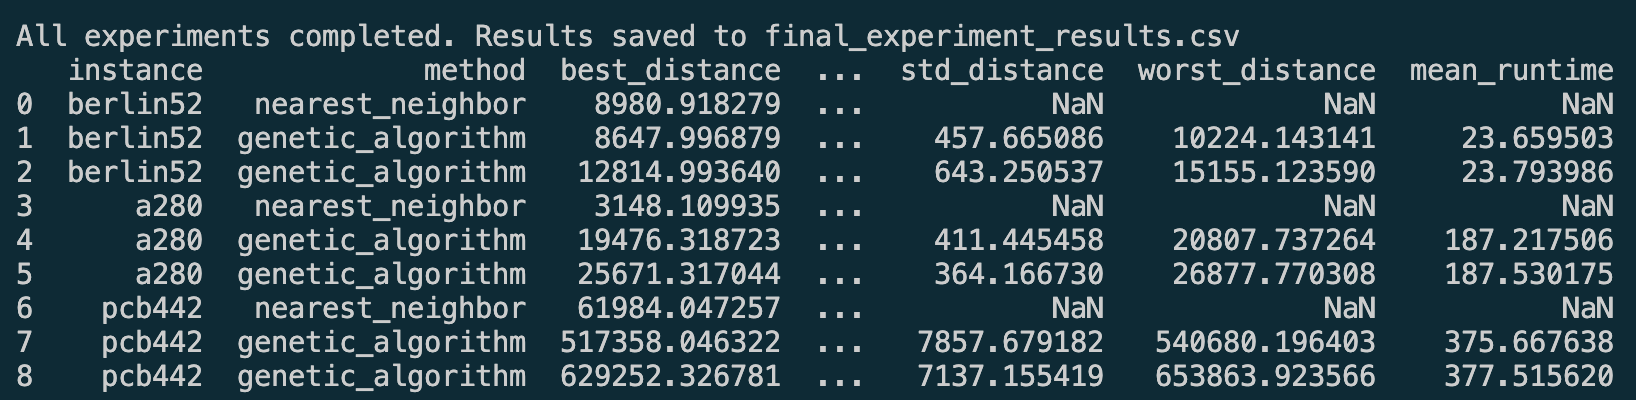
\includegraphics[width=0.45\textwidth]{figures/group_data.png}
    \caption{Convergence of GA across datasets.}
    \label{fig:convergence}
\end{figure}

\begin{figure}[h]
    \centering
    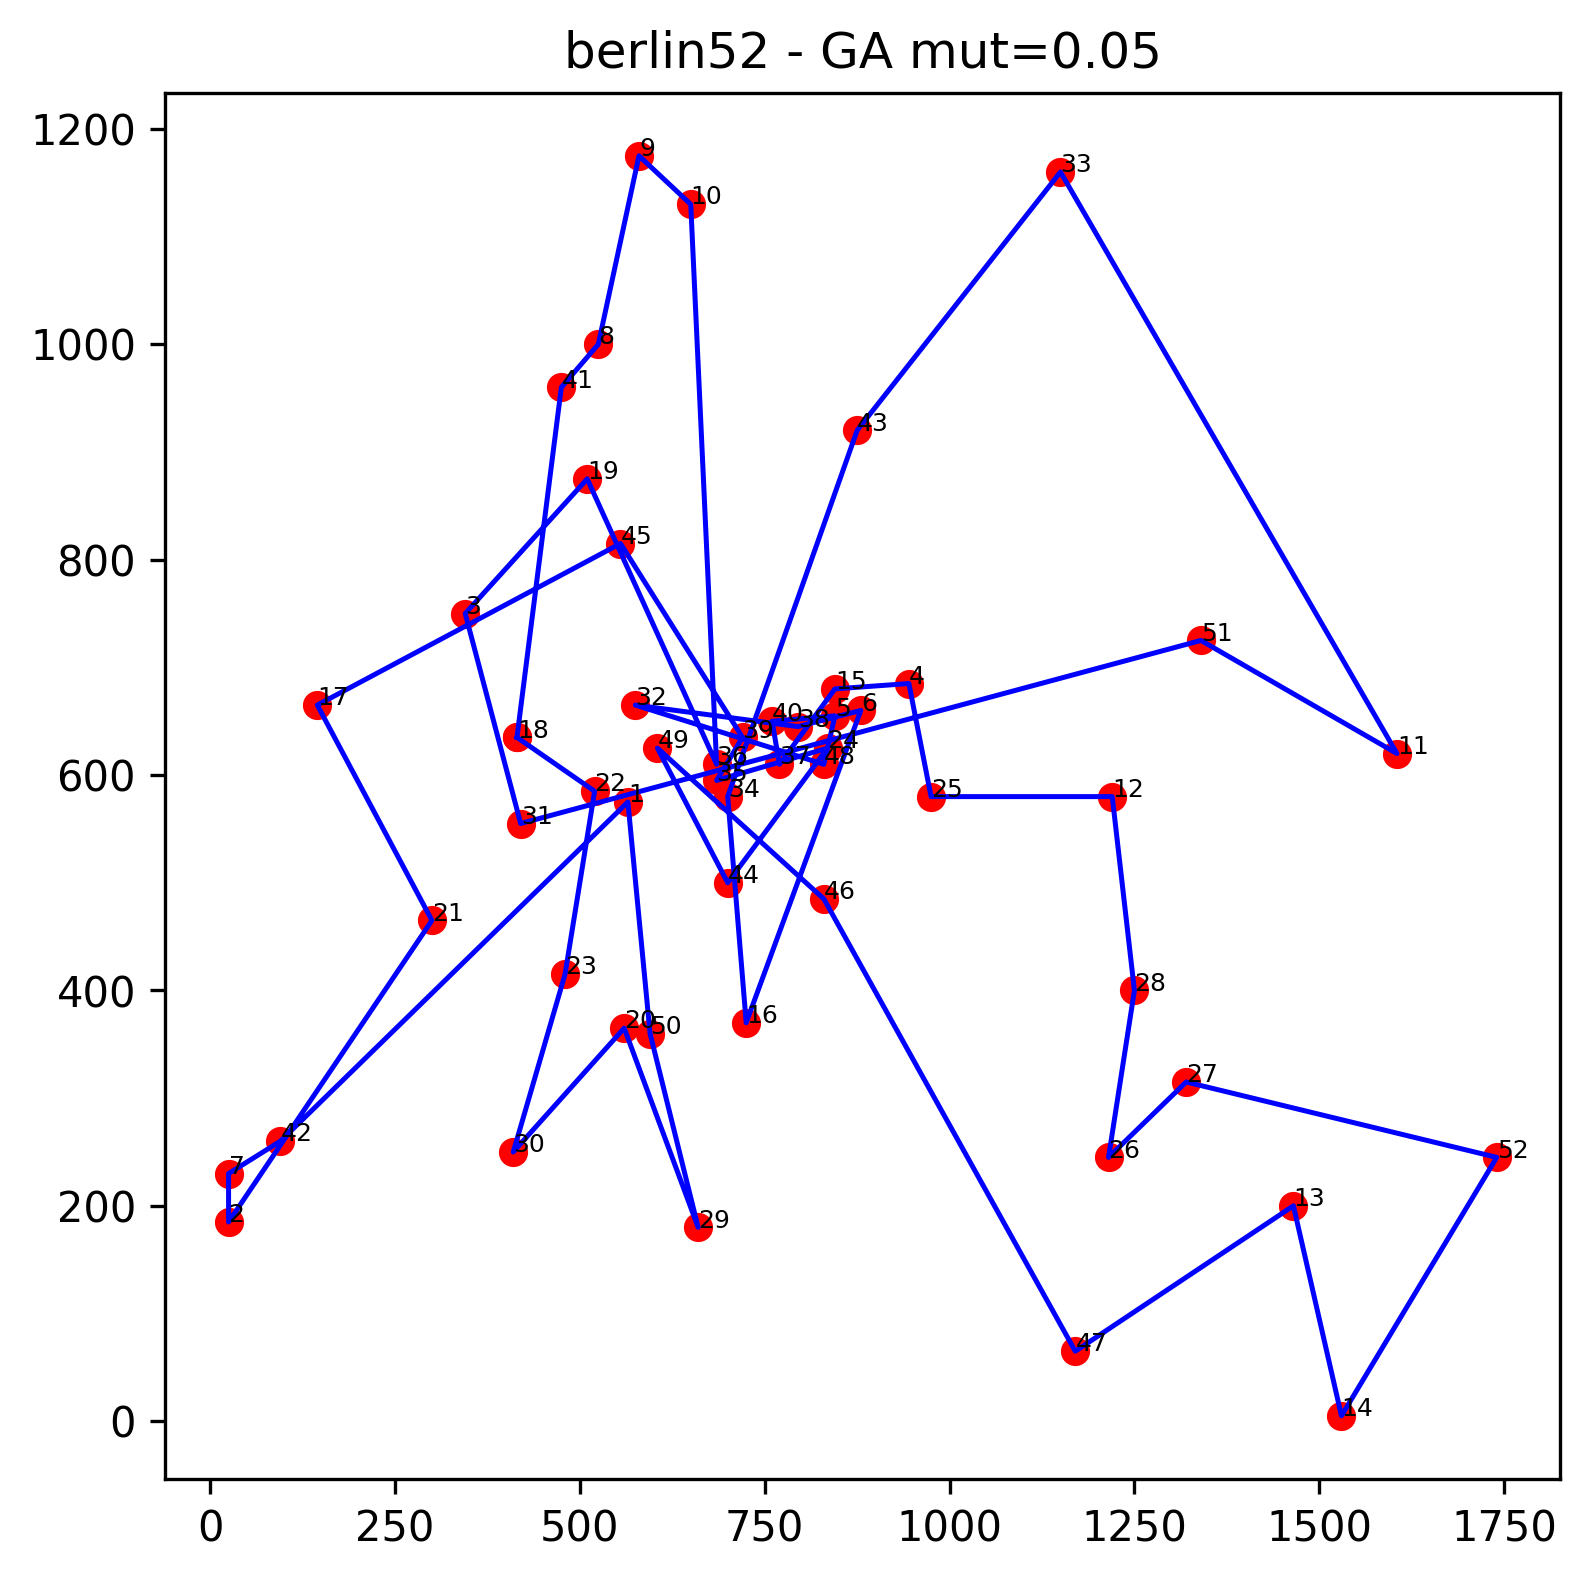
\includegraphics[width=0.45\textwidth]{figures/berlin52_ga_mut0.05.png}
    \caption{Best GA route for berlin52 instance.}
    \label{fig:route52}
\end{figure}

\begin{figure}[h]
    \centering
    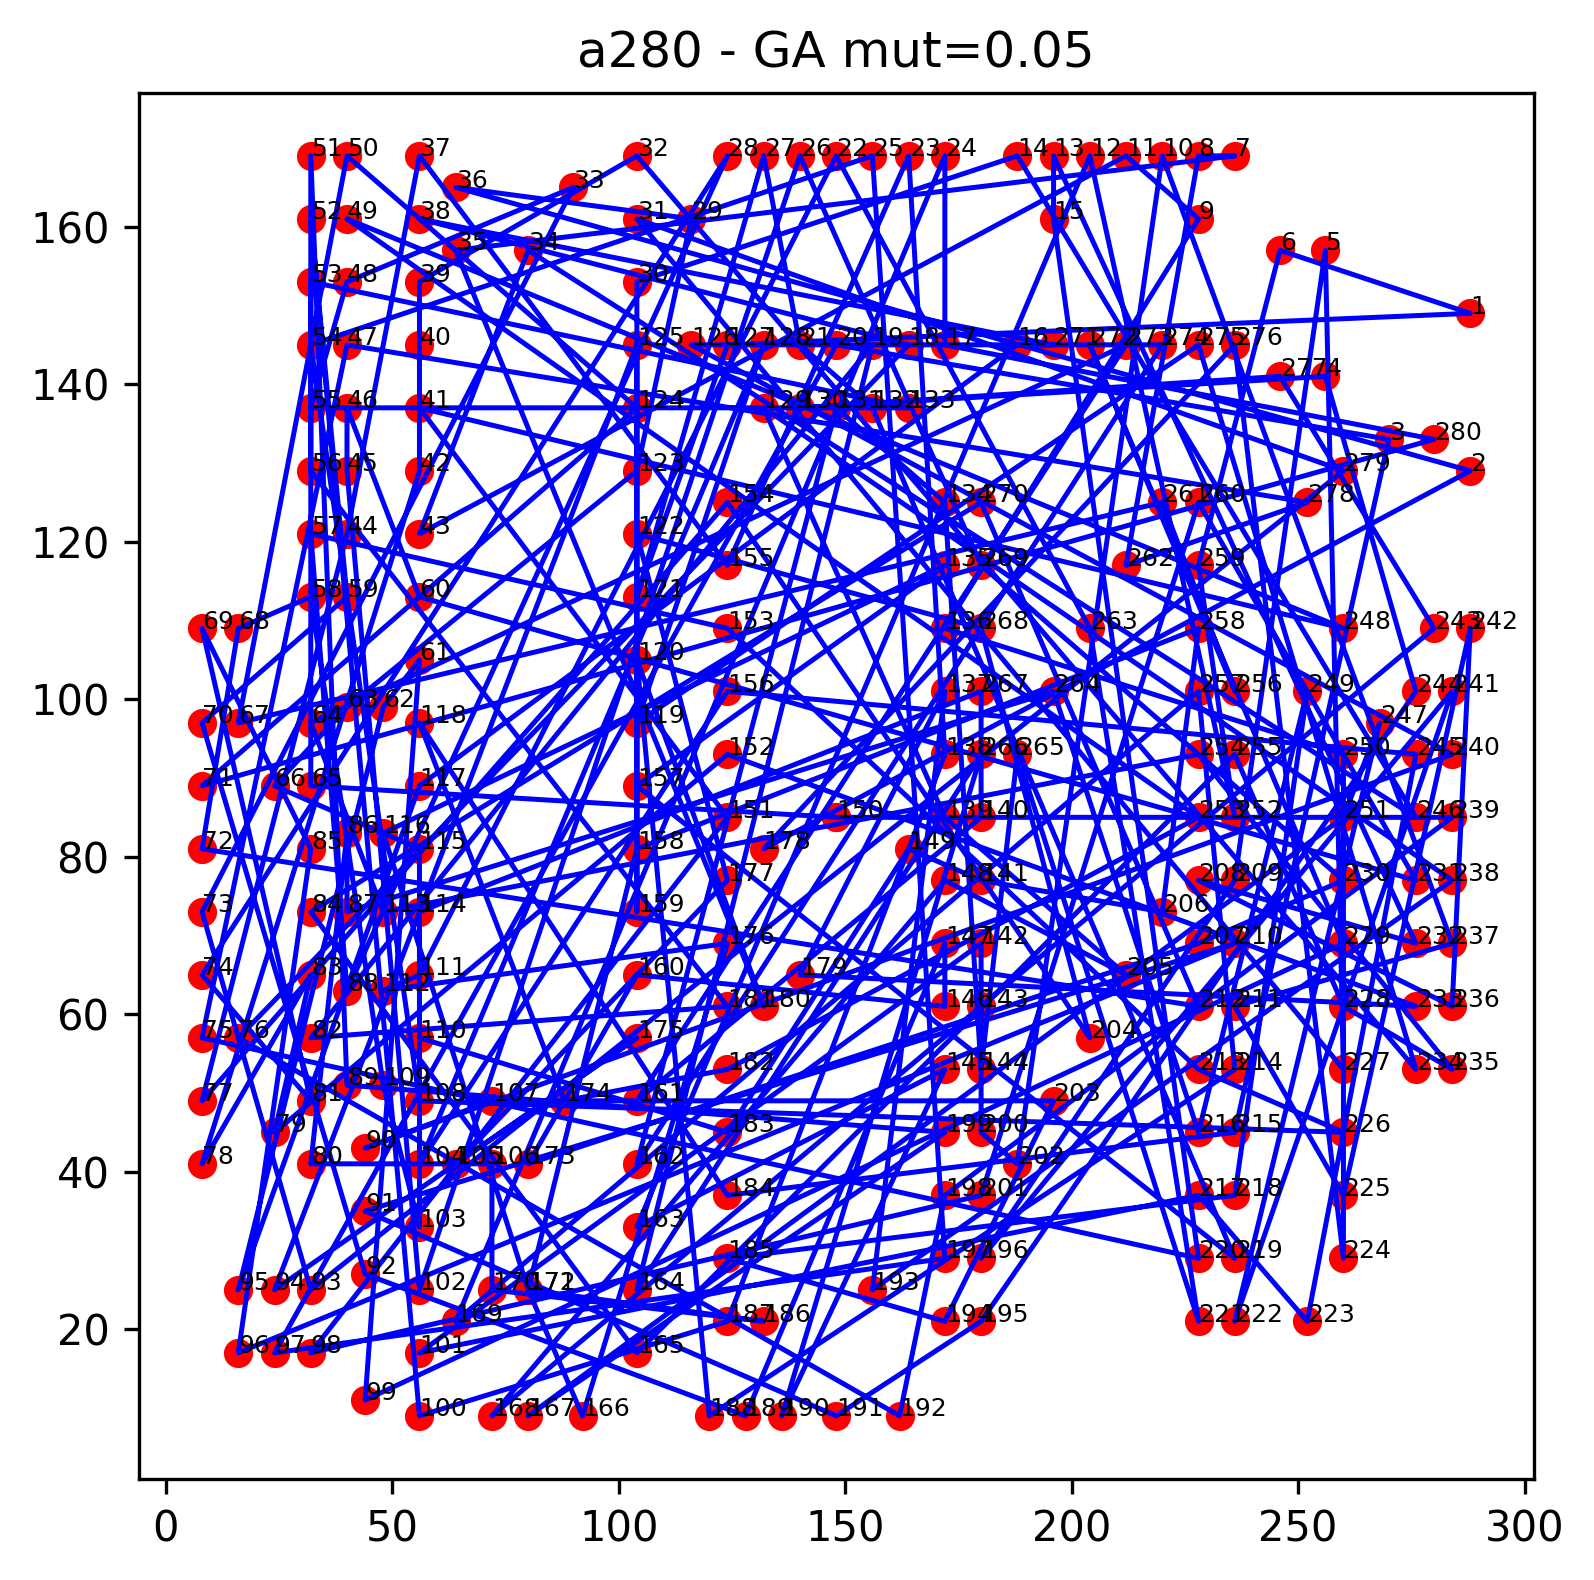
\includegraphics[width=0.45\textwidth]{figures/a280_ga_mut0.05.png}
    \caption{Best GA route for a280 instance.}
    \label{fig:route280}
\end{figure}

\begin{figure}[h]
    \centering
    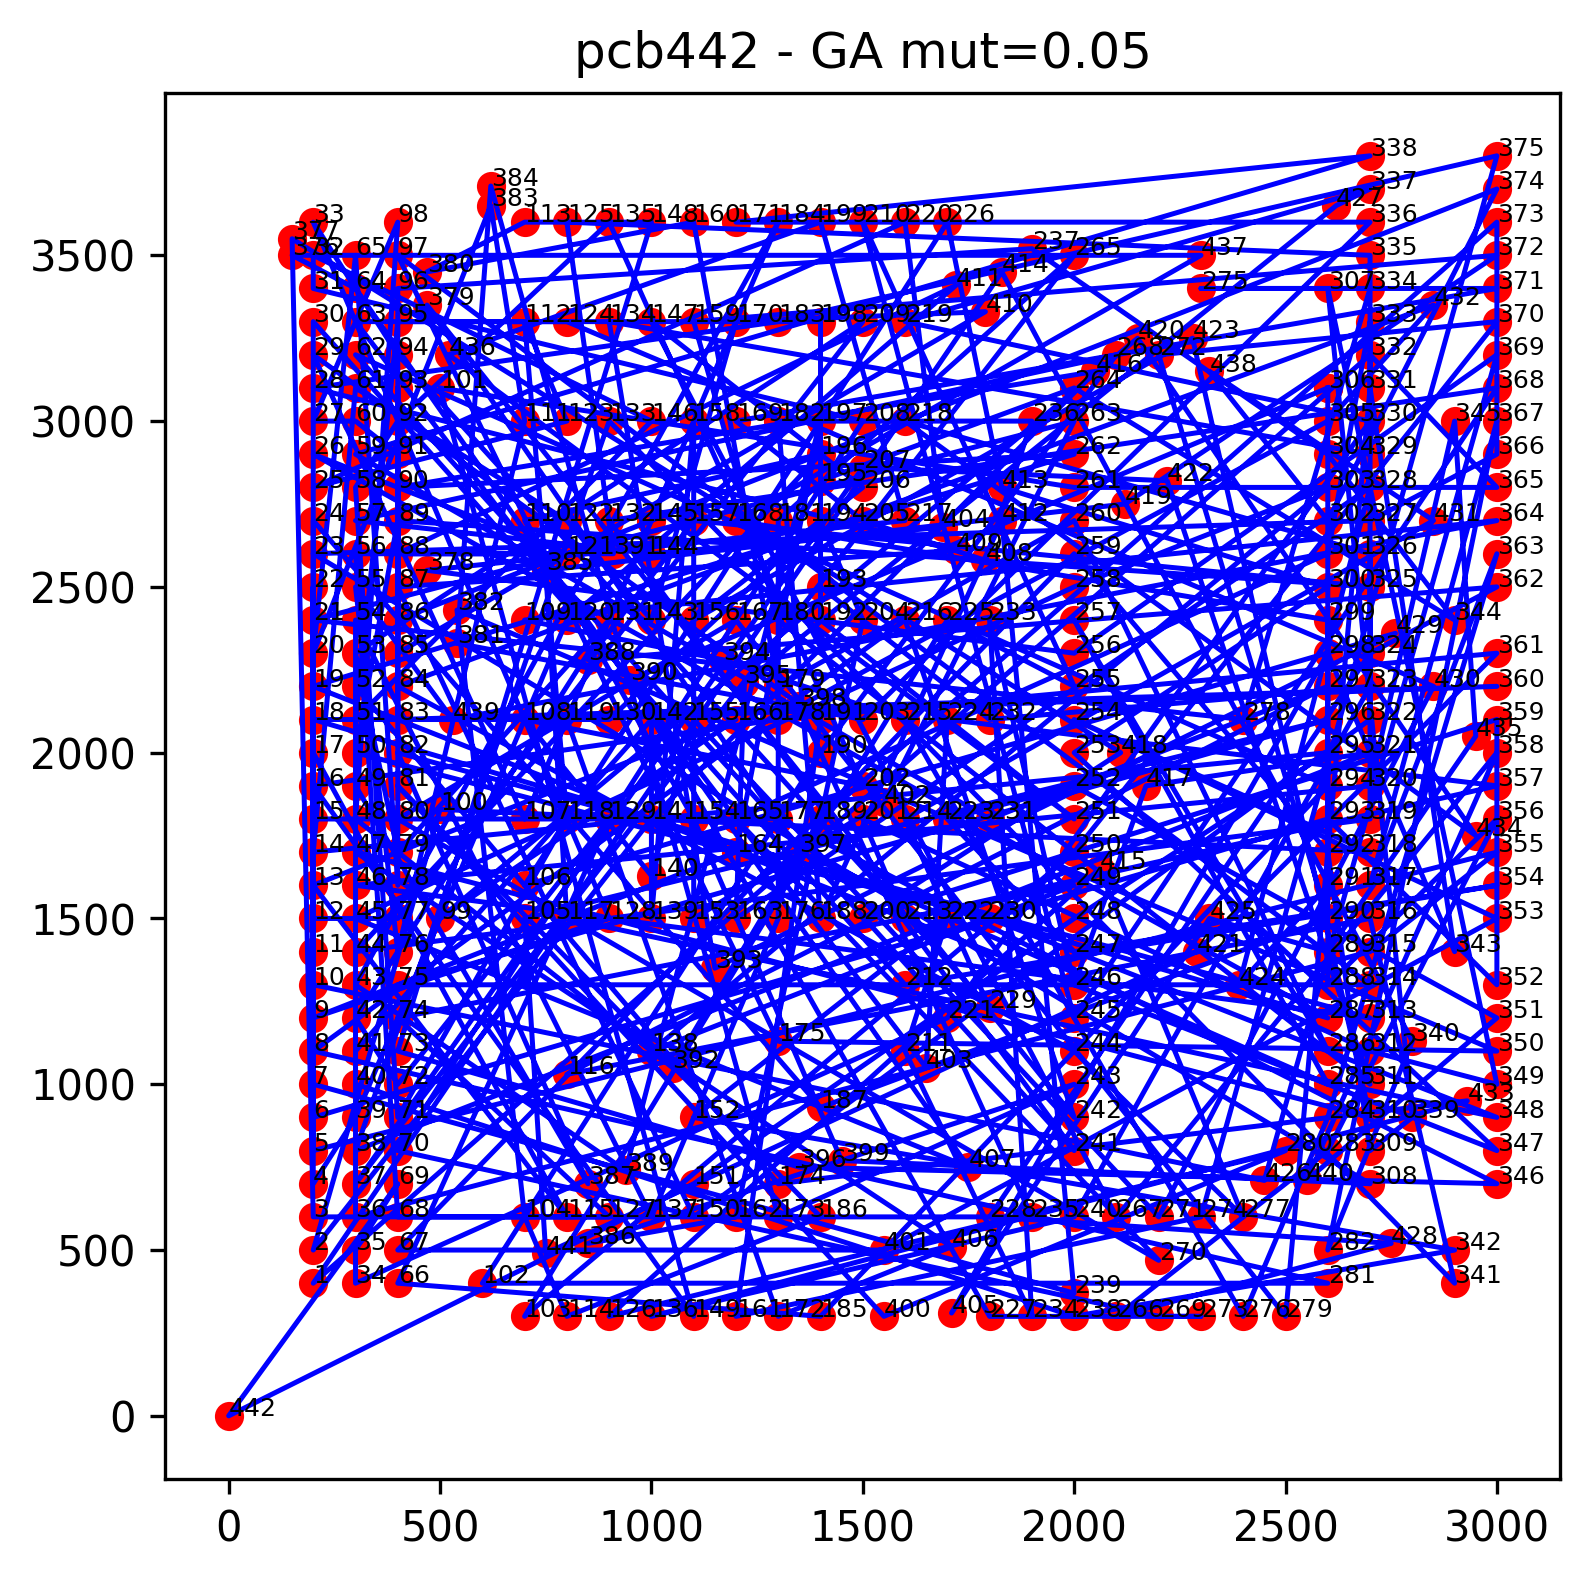
\includegraphics[width=0.45\textwidth]{figures/pcb442_ga_mut0.05.png}
    \caption{Best GA route for pcb442 instance.}
    \label{fig:route280}
\end{figure}

\section{Conclusions and Future Work}
\subsection{Major takeaways}
\begin{itemize}
    \item GA achieved modest success on small instances but performed poorly on medium and large ones.
    \item Mutation rate was critical: lower mutation (0.01) consistently outperformed higher mutation (0.05).
    \item Nearest neighbor surprisingly outperformed GA for larger instances.
\end{itemize}

\subsection{Future directions}
\begin{itemize}
    \item Integrating local search (e.g., 2-opt or 3-opt) as a hybrid GA could drastically improve results.
    \item Adaptive mutation rates could balance exploration/exploitation dynamically.
    \item Parallel implementations would reduce runtimes for larger datasets.
    \item Testing against additional heuristics (Ant Colony, Lin–Kernighan) would provide broader benchmarks.
\end{itemize}

\bibliography{refs}

\begin{thebibliography}{1}
\bibitem{wikiTSP} Wikipedia contributors, ``Travelling salesman problem,'' \emph{Wikipedia}, 2025. [Online]. Available: \url{https://en.wikipedia.org/wiki/Travelling_salesman_problem}
\end{thebibliography}

\end{document}